\chapter{Platforma od strony technicznej}
\label{chapter:platform-technical}
Ogólny schemat platformy wraz z użytymi technologiami został przedstawiony na rysunku \ref{fig:platform-schema}.

\begin{figure}[h]
    \centering
    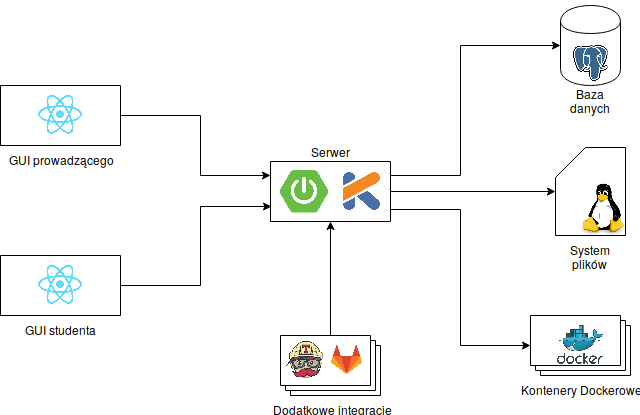
\includegraphics[width = 13cm]{chapter05/platform_schema.png}
    \caption{Schemat platformy i użytych technologii (źródło własne).}
    \label{fig:platform-schema}
\end{figure}

Platforma składa się z dwóch webowych interfejsów graficznych: interfejsu prowadzącego oraz studenta.
Oba interfejsy zostały napisane w technologii ReactJS z użyciem biblioteki MaterialUI.

Moduł serwera został napisany w języku Kotlin z wykorzystaniem SpringBoot’a w~wersji 2.0.

Serwer przechowuje dane w dwóch formach: rekordów w bazie danych oraz plików.
Metadane, takie jak termin realizacji wskazanego etapu lub grupy projektowe, do których są przypisani studenci, są zapisywane w bazie PostgreSQL.
Schematy tabel i ich relacji zostały omówione w podrozdziale \ref{database}.
Dane w postaci plików są przechowywane na dysku serwera w systemie plików Linux.
W podrozdziale \ref{directories} opisano użyte struktury katalogów.

Programy studentów są uruchamiane w kontenerach Dockerowych.
Proces testowania aplikacji studentów został opisany w sekcji \ref{run-and-test}.
Kolejny podrozdział omawia utworzenie nowego środowiska uruchomieniowego w postaci pliku konfiguracyjnego Dockerfile.

Opis zastosowanej autoryzacji i autentykacji użytkowników można znaleźć w podrozdziale \ref{authorization}.

Przykład konfiguracji i uruchomienia platformy na dowolnym serwerze został omówiony w ramach sekcji \ref{run-platform}.

Platformę można zintegrować z zewnętrznymi narzędziami.
Przykładem takiej integracji może być powiązanie z systemem Continuous Integration (na przykład Travis).
Taki system można skonfigurować tak, aby w ramach testów automatycznych budował program, wysyłał plik wykonywalny do platformy i raportował o wyniku uruchomienia.
Przykład takiej integracji platformy z zewnętrznym narzędziem został opisany w~podrozdziale \ref{ci-integration}.

\section{Schemat bazy}
\label{database}

\begin{figure}[h]
    \centering
    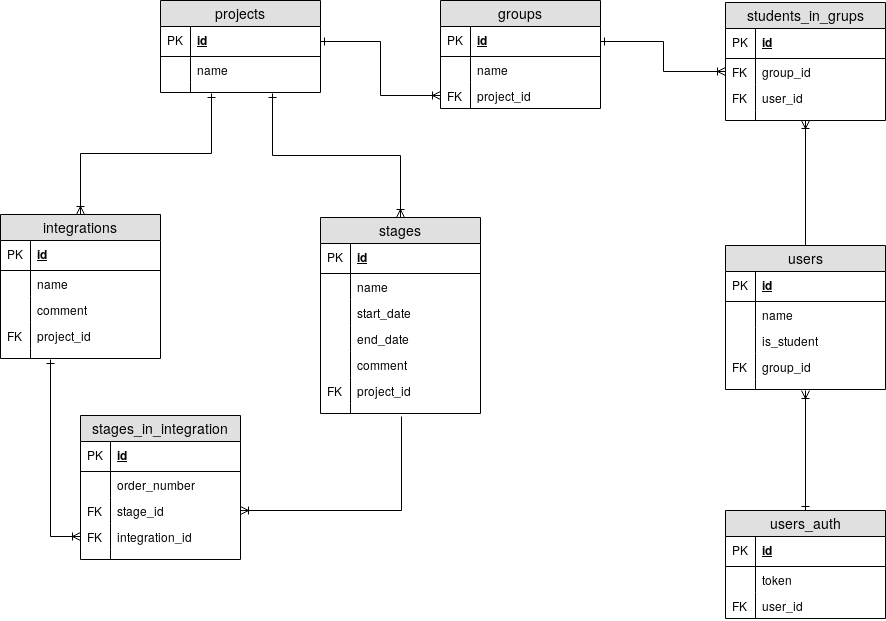
\includegraphics[width = 13cm]{chapter05/db_schema.png}
    \caption{Schemat bazy danych (źródło własne).}
    \label{fig:platform-db-schema}
\end{figure}

Schemat tabel i relacji bazodanowych utworzony w ramach pracy znajduje się na rysunku \ref{fig:platform-db-schema}.
Do przechowywania metadanych wykorzystano osiem tabel.
W przedstawionych strukturach zapisywane są informacje o:
\begin{itemize}
    \item projektach (grupach, etapach i integracjach w ramach projektu)
    \item studentach (ich przynależności do grup i tokenach autoryzacyjnych)
    \item prowadzących (i ich tokenach autoryzacyjnych)
\end{itemize}

Do przechowywania danych użyto relacyjnej bazy PostgreSQL w wersji 12 beta 1.
Pełne definicje tabel wraz z użytymi typami danych i więzami znajdują się w załączniku~\ref{file:database-schema}.


\section{Schemat katalogów plików}
\label{directories}

\begin{figure}[h]
    \centering
    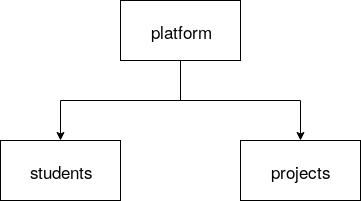
\includegraphics[width = 6cm]{chapter05/platform_main_dirs.png}
    \caption{Główny schemat katalogów (źródło własne).}
    \label{fig:platform-main-directories}
\end{figure}

Główny schemat katalogów plików znajduje się na rysunku \ref{fig:platform-main-directories}.
Można wyróżnić na nim dwa podstawowe foldery: \textit{students} oraz \textit{projects}.
Wewnątrz pierwszego z nich zapisywane są wszystkie dane i pliki związane z aktywnością studentów zarejestrowaną na platformie.
Do zapamiętywanych informacji należą: zamieszczane raporty, linki do kodu, programy oraz logi z przebiegu aplikacji i wyniki przeprowadzonych testów akceptacyjnych.
Drugi folder zawiera definicje projektów wraz z etapami i integracjami oraz utworzone przez prowadzących przypadki testowe.

Na rysunkach \ref{fig:projects-directories} i \ref{fig:students-directories} zostały zamieszone odpowiednio schematy katalogów wewnątrz folderów \textit{projects} oraz \textit{students}.
Dla obu schematów zostały wyróżnione pliki i foldery, które nie występują pojedynczo w ramach katalogów.
W miejscu zbiorczej nazwy oznaczonej jako ${nazwa\_katalogu}_{i}$ na schemacie należy rozumieć docelową nazwę folderu.

\begin{figure}[H]
    \centering
    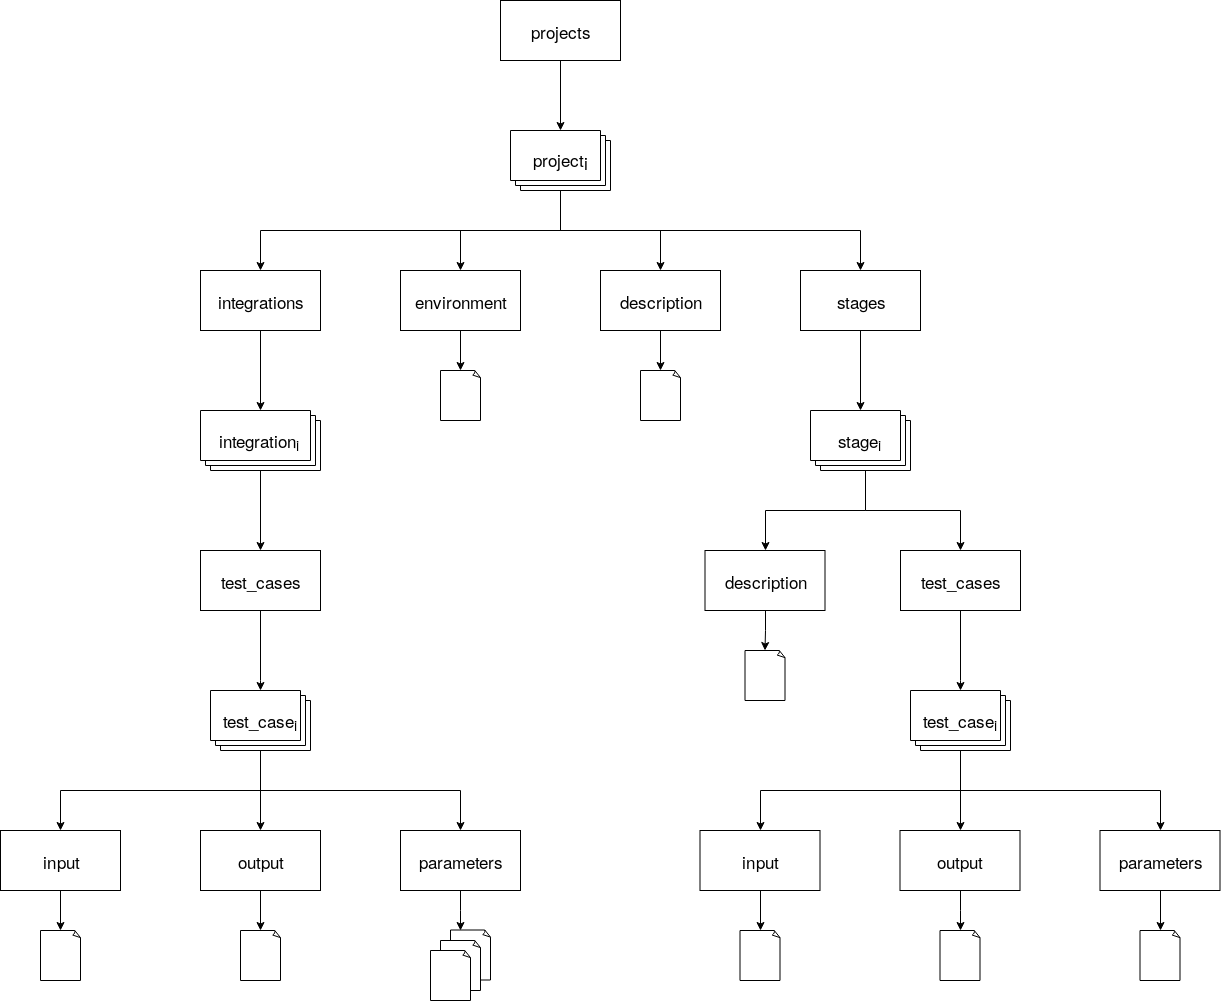
\includegraphics[width = 13cm]{chapter05/projects_dirs.png}
    \caption{Schemat katalogów i plików wewnątrz folderu projects (źródło własne).}
    \label{fig:projects-directories}
\end{figure}

\begin{figure}[H]
    \centering
    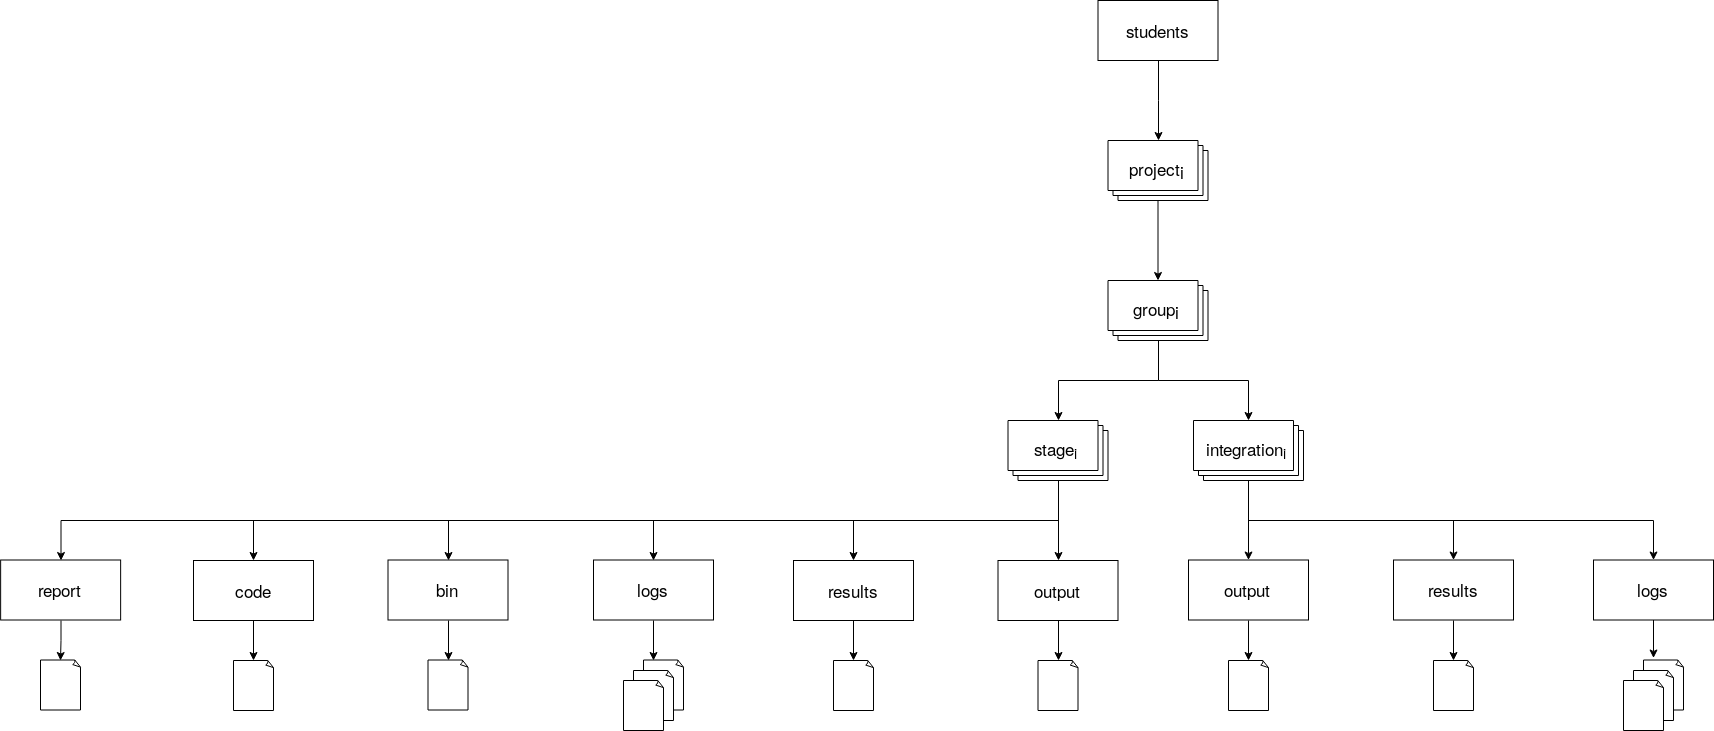
\includegraphics[width = 13cm]{chapter05/students_dirs.png}
    \caption{Schemat katalogów i plików wewnątrz folderu students (źródło własne).}
    \label{fig:students-directories}
\end{figure}

\section{Uruchomianie i testowanie programów studentów}
\label{run-and-test}

Programy studentów są uruchamiane w kontenerach Dockerowych.
Obraz środowiska jest ustalany dla zadanego projektu poprzez plik konfiguracyjny Dockerfile (patrz podrozdział \ref{environment_configuration}).

Technologia Docker jest szeroko używana komercyjnie.
Dzięki temu charakteryzuje się ona wysoką niezawodnością i stabilnością.
Również biblioteki OpenSource ułatwiające uruchamianie kontenerów Dockerowych bezpośrednio z kodu Javowego są szeroko stosowane i dobrze przetestowane.
Samo uruchamianie kontenerów, ich integracja oraz konfiguracja nowych środowiska jest szybka i stosunkowo prosta.

\begin{figure}[h]
    \centering
    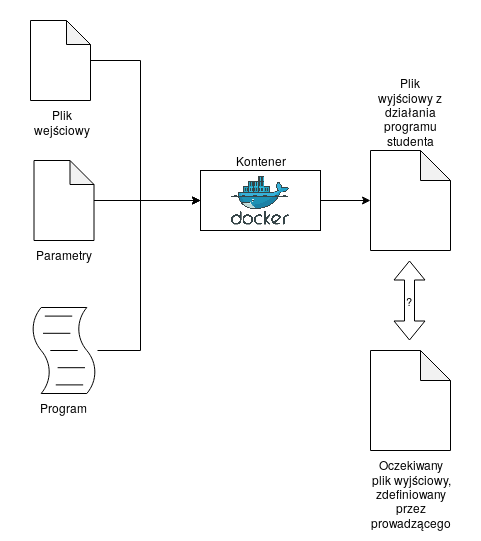
\includegraphics[width = 7cm]{chapter05/single_test_case.png}
    \caption{Schemat wykonania pojedynczego przypadku testowego w ramach etapu (źródło własne).}
    \label{fig:single-test-case}
\end{figure}

Poprzez naciśnięcie na platformie przycisku \textit{PLAY} dla wybranej aplikacji studenckiej uruchamiane są kolejno wszystkie zdefiniowane przypadki testowe dla zadanego etapu.
Schemat wykonania pojedynczego przypadku testowego w ramach etapu dla programu studentów został przedstawiony na rysunku \ref{fig:single-test-case}.
Uruchomienie pojedynczego przypadku testowego sprowadza się do utworzenia nowego kontenera Dockerowego i podania mu odpowiednich ścieżek do:
\begin{itemize}
    \item programu studenta, dla którego ma zostać uruchomiony dany przypadek testowy,
    \item pliku definiującego dane wejściowe dla zadanego przypadku testowego (pliku wejściowego),
    \item pliku definiującego parametry wejściowe dla programu (pliku z parametrami),
    \item pliku wyjściowego, do którego zapisany zostanie rezultat wykonania danego przypadku testowego.
\end{itemize}
Zarówno utworzenie kontenera, jak i załączenie odpowiednich ścieżek do plików jest wykonywane automatycznie przez platformę.

W celu ustalenia poprawności działania aplikacji dla zadanego przypadku testowego platforma dokonuje porównania otrzymanego w wyniku przebiegu testu pliku wyjściowego ze zdefiniowanym w ramach przypadku testowego oczekiwanym plikiem wyjściowym.
Jeśli obie dane są zgodne, działanie programu dla wykonywanego testu uważa się za prawidłowe.

Platforma zlicza również liczbę zaliczonych testów w ramach etapu.
Jeśli rezultaty dla wszystkich przypadków testowych są prawidłowe, to program uznaje się za ukończony w ramach danego zadania.

\begin{figure}[h]
    \centering
    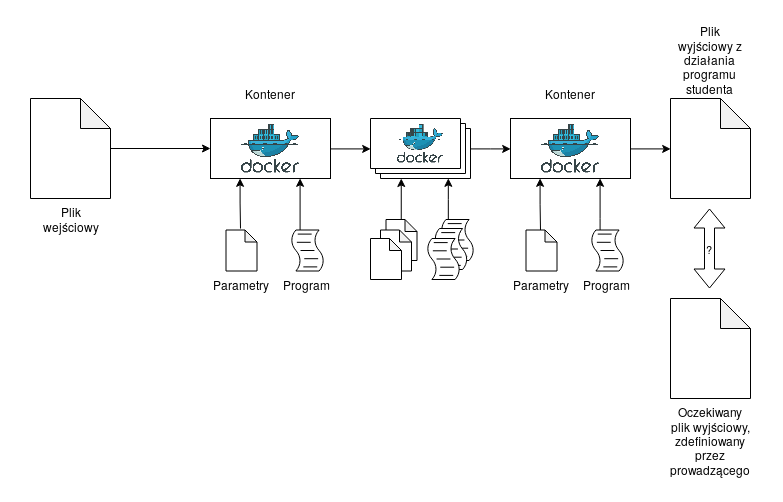
\includegraphics[width = 12cm]{chapter05/integration.png}
    \caption{Schemat wykonania pojedynczego przypadku testowego w ramach procesu integracji (źródło własne).}
    \label{fig:integration}
\end{figure}

Poprzez naciśnięcie na platformie przycisku \textit{PLAY} dla wybranego procesu integracji uruchamiane są kolejno wszystkie zdefiniowane dla niego przypadki testowe.
Schemat wykonania pojedynczego przypadku testowego w ramach procesu integracji został przedstawiony na rysunku \ref{fig:integration}.
Przebieg procesu integracji jest podobny do wykonania pojedynczego przypadku testowego.
Różnica polega na tym, że w ramach tego zadania uruchamiane jest kolejno kilka programów studentów dla zdefiniowanych przez prowadzącego etapów integracji.
Plik wyjściowy utworzony w wyniku uruchomienia etapu jest plikiem wejściowym dla kolejnego, następującego po nim.
W celu oceny poprawności wykonania przypadku testowego oczekiwany plik wyjściowy zdefiniowany dla procesu integracji jest porównywany z plikiem wyjściowym dla ostatniego etapu w ramach badanego procesu integracji.

Aby uniknąć nieprawidłowego i niekontrolowanego zachowania programów studentów został wprowadzony ograniczony czas ich wykonania.
Ten okres dla każdego, pojedynczego przypadku testowego wynosi pięć sekund.
Po tym czasie kontener uruchamiający przypadek testowy jest zatrzymywany i test kończy się automatycznie.
Rezultat przerwanego testu uważa się za nieprawidłowy.
Dzięki takiemu rozwiązaniu można uniknąć między innymi wyczerpania zasobów sprzętowych dla platformy w wyniku uruchamiania programów zawierających nieskończone pętle.


\section {Konfiguracja środowiska uruchomieniowego}
\label{environment_configuration}

Dla każdego projektu należy zdefiniować środowisko, na jakim uruchamiane mają być programy studentów.
Konfiguracja odbywa się poprzez załączenie dla projektu odpowiednio sformułowanego pliku Dockerfile.

Przykład poprawnie zdefiniowanego środowiska dla systemu Linux z zainstalowaną Javą w wersji 8 został przedstawiony poniżej:

{\fontfamily{qcr}\selectfont
\tiny
\begin{lstlisting}

    FROM openjdk:8-alpine

    CMD ["java", "-jar", "/home/app", "/home/input.txt", "/home/parameters.txt", "/home/output.txt"]

\end{lstlisting}
}

Przykład poprawnie zdefiniowanego środowiska dla systemu Linux i języka C wygląda następująco:

TODO: fix c dockerfile
{\fontfamily{qcr}\selectfont
\tiny
\begin{lstlisting}

    FROM openjdk:8-alpine

    CMD ["gcc", "./home/app", "/home/input.txt", "/home/parameters.txt", "/home/output.txt"]

\end{lstlisting}
}

Komenda \textit{FROM} definiuje obraz systemu jaki ma zostać użyty do stworzenia środowiska.
\textit{CMD} opisuje polecenie uruchomienia programu wraz z przyjmowanymi parametrami.
Powyższe pliki są poprawnymi plikami konfiguracyjnymi dla kontenerów Docker'owych.
Dokładny opis tworzenia prawidłowych i bardziej złożonych plików Dockerfile można znaleźć w dokumentacji dla narzędzia Docker \cite{docker-config}.

Platforma akceptuje dowolny plik Dockerfile, który opiera komendę uruchomienia programu na czterech następujących ścieżkach:
\begin{itemize}
    \item \textit{/home/app} - ścieżka do programu studentów wewnątrz kontenera,
    \item \textit{/home/input.txt} - ścieżka do pliku wejściowego dla przypadku testowego wewnątrz kontenera,
    \item \textit{/home/parameters.txt} - ścieżka do parametrów wywołania programu dla przypadku testowego wewnątrz kontenera,
    \item \textit{/home/output.txt} - ścieżka do pliku wyjściowego dla przypadku testowego wewnątrz kontenera.
\end{itemize}

W trakcie wykonywania przypadku testowego platforma kopiuje odpowiednie pliki pod wskazane ścieżki wewnątrz kontenera, stąd podane wyżej parametry powinny być niezmienne w ramach wszystkich Dockerfile.
Warto zaznaczyć, że omawiany plik konfiguracyjny nie jest walidowany przez platformę podczas załączania do projektu.


\section {Uwierzytelnianie użytkowników}
\label{authorization}

Uwierzytelnianie użytkowników odbywa się przy pomocy serwisu GitHub \cite{gitHub}.
Jest to najpopularniejsza platforma hostingowa przeznaczona dla repozytoriów gitowych, która posiada otwarte API (ang. Application Programming Interface).
Uwierzytelnianie przy użyciu zweryfikowanego źródła jest zarówno łatwiejsze od strony technicznej, jak i bezpieczniejsze dla użytkowników.
W ramach platformy nie ma potrzeby przechowywania i~zabezpieczania wrażliwych danych użytkowników, jakimi są prywatne hasła.

Najpopularniejszym sposobem identyfikacji użytkownika jest porównanie jego adresu e-mail.
Przy zastosowaniu takiego typu uwierzytelnienia wymagane od użytkowników (studentów i prowadzących) jest posiadanie konta na githubie z dodanym e-mailem uczelnianym (lub innym adresem znanym przez prowadzącego).
Warto tutaj zaznaczyć, że do konta na githubie może być dodanych wiele adresów e-mail.
Dodanie nowego adresu nie wpływa negatywnie na sposób korzystania z konta github przez użytkowników.

Proces uwierzytelniania można podzielić na następujące kroki:
\begin{enumerate}
\item Użytkownik naciska przycisk \textit{Zaloguj} na interfejsie webowym platformy.
\item Aplikacja webowa przekierowuje użytkownika na stronę GitHub, na której loguje się on do serwisu i nadaje odpowiednie uprawnienia do odczytu danych platformie.
\item Aplikacja webowa otrzymuje tymczasowy kod dostępu z GitHub odpowiadający profilowi zalogowanego użytkownika.
\item Aplikacja webowa przekazuje kod dostępu do serwera.
\item Serwer odpytuje GitHub o token dla użytkownika na podstawie otrzymanego z~aplikacji webowej kodu dostępu.
\item Serwer odpytuje GitHub o adresy mailowe przypisane do konta użytkownika o~zadanym tokenie.
\item Serwer filtruje otrzymane maile i sprawdza, czy któryś z nich jest zgodny z mailem użytkownika (nazwą) zapisanym w bazie.
\item Jeśli tak to odsyłana jest do użytkownika informacja zwrotna zawierająca token, a~zweryfikowany użytkownik przekierowywany jest na odpowiedni dla jego uprawnień ekran (widok projektu w przypadku studenta lub widok wyboru podglądu albo zarządzania projektami w przypadku prowadzącego).
\end{enumerate}

Serwis w miarę potrzeby może zweryfikować czy dany użytkownik jest studentem czy prowadzącym.
Poziom uprawnień dla użytkownika jest zapisywany i odczytywany z bazy z tabeli \textit{Users}.
Więcej informacji o procesie uwierzytelniania przez GitHub, implementacji i bezpieczeństwie takiego rozwiązania można znaleźć w dokumentacji \cite{gitHub-auth-basic} i \cite{gitHub-oauth-app}.

Uwierzytelnienie jest potrzebne do dostępu do platformy i wykonywania zapytań.
Przykładowo użytkownik będący studentem nie ma uprawnień do usunięcia projektu i~nie może wykonać takiej akcji.
Prowadzący jest traktowany jako administrator i ma dostęp do wszystkich akcji studenta.
Dodatkowo ma on uprawnienia do definicji i edycji projektu oraz podglądu statystyk z uruchomienia etapów oraz integracji.

\section {Zestawienie platformy na serwerze}
\label{run-platform}

TODO: Opis i przykład

- zmienne systemowe TEST\_PLATFORM\_CLIENT\_ID, TEST\_PLATFORM\_SECRET
- secret - nie powinien być publicznie udostępniany
- strona startowa i callback
- nadawane przez github
- strona do rejestracji aplikacji []

\section {Przykład integracji platformy z narzędziem CI oraz repozytorium kodu}
\label{ci-integration}

TODO: opis i przykład integracji platformy z narzędziem CI oraz repozytorium
kodu.